\documentclass{article}
\usepackage{hyperref}
\usepackage{listings}
\usepackage{color}
\usepackage{xcolor}
\usepackage{geometry}
\usepackage{graphicx}
\usepackage{amsmath}
\usepackage{caption}
\usepackage{subcaption}
\usepackage[capitalise]{cleveref}
\usepackage{wrapfig}
\usepackage{amssymb}

\geometry{margin=1in}
\pdfminorversion=6

\newcommand\TODO[1]{\textcolor{red}{TODO: #1}}

\newcommand\header[2]{
    \begin{center}
        {\large
        UCSD CSE 167 Assignment #1: \\
        \vspace{0.3cm}
        \Large
        #2}
    \end{center}
}

\definecolor{dkgreen}{rgb}{0,0.6,0}
\definecolor{gray}{rgb}{0.5,0.5,0.5}
\definecolor{mauve}{rgb}{0.58,0,0.82}
\lstset{frame=tb,
        aboveskip=3mm,
        belowskip=3mm,
        showstringspaces=false,
        columns=flexible,
        basicstyle={\small\ttfamily},
        numbers=none,
        numberstyle=\tiny\color{gray},
        keywordstyle=\color{blue},
        commentstyle=\color{dkgreen},
        stringstyle=\color{mauve},
        breaklines=true,
        breakatwhitespace=true,
        tabsize=2
}

% Taken from https://tex.stackexchange.com/questions/83085/how-to-improve-listings-display-of-json-files

\colorlet{punct}{red!60!black}
\definecolor{delim}{RGB}{20,105,176}
\colorlet{numb}{magenta!60!black}

\lstdefinelanguage{json}{
    basicstyle=\normalfont\ttfamily,
    numberstyle=\scriptsize,
    stepnumber=1,
    numbersep=8pt,
    showstringspaces=false,
    breaklines=true,
    frame=lines,
    tabsize=2,
    literate=
     *{0}{{{\color{numb}0}}}{1}
      {1}{{{\color{numb}1}}}{1}
      {2}{{{\color{numb}2}}}{1}
      {3}{{{\color{numb}3}}}{1}
      {4}{{{\color{numb}4}}}{1}
      {5}{{{\color{numb}5}}}{1}
      {6}{{{\color{numb}6}}}{1}
      {7}{{{\color{numb}7}}}{1}
      {8}{{{\color{numb}8}}}{1}
      {9}{{{\color{numb}9}}}{1}
      {:}{{{\color{punct}{:}}}}{1}
      {,}{{{\color{punct}{,}}}}{1}
      {\{}{{{\color{delim}{\{}}}}{1}
      {\}}{{{\color{delim}{\}}}}}{1}
      {[}{{{\color{delim}{[}}}}{1}
      {]}{{{\color{delim}{]}}}}{1},
}

\hypersetup{colorlinks=true}


\begin{document}

\header{1}{2D Graphics}
\setcounter{section}{-1}

\begin{figure}[ht]
    \centering
    \caption{Images we will produce in this homework.}
    \label{fig:teaser}
\end{figure}

Computer graphics is the field that studies how to process \emph{visual data}, such as shapes, volumes, and lights. \textbf{Images} are an important class of visual data: they can be the pictures recorded by the camera of your cellphone or a DSLR, outputs of video games or movie visual effects, legends and arrows on Google map telling you where to go next, or visualization of the radio waves coming from a black hole. An important subfield of computer graphics, rendering, studies the generation of images.

\begin{figure}[h]
    \centering
    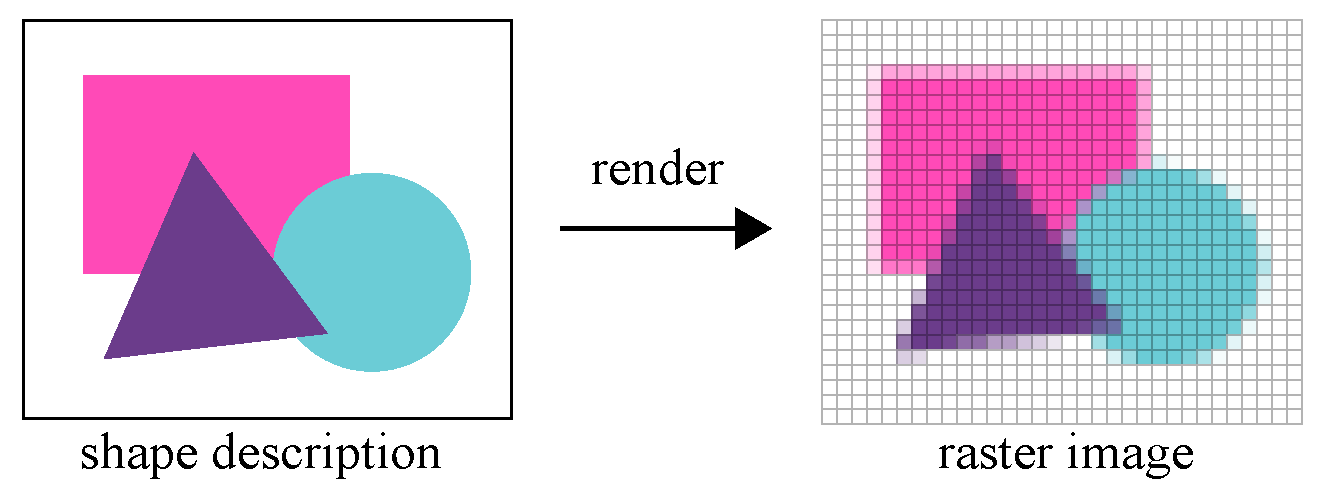
\includegraphics[width=0.6\linewidth]{imgs/render2d.pdf}
    \caption{In this homework, we will render a set of 2D shapes into a raster image.}
    \label{fig:render2d}
\end{figure}

In our first homework, we will implement a 2D renderer that takes a set of simple shapes (circle, squares, and triangles), and turn them into a raster image (\cref{fig:render2d}). A raster image is a particular kind of image that represent 2D contents using a grid of \emph{pixels}, where each pixel denotes the color at that location. Raster images are convienient because our displays (and our camera sensor) usually also represent images as a grid of pixels.

Before you start coding, we recommend you to go through the whole handout to have some ideas of what needs to be done.

\paragraph{Submission.} Submit your code and the outputs of your code through Canvas. In addition, for the quizzes below, answer them through the Gradescope (you can access it through Canvas).

\paragraph{Grading.} We will compare your outputs to our reference solutions. The points of the quizes are included in the total points on the section titles.

\paragraph{Colloboration policy.} We expect you to write the code on your own. Feel free to discuss between the peers and ask us questions though!

\section{Building Balboa}

We are going to build our code on top of a currently barebone codebase \emph{balboa}. Balboa already includes all the third party libraries (stb\_image, stb\_image\_write, and json) in its repository.
All you need to do is to clone the repo and build it using CMake (assuming you are in a Unix-like system):
\begin{lstlisting}[language=bash]
  git clone https://github.com/BachiLi/balboa_public
  mkdir build
  cd build
  cmake ..
  make -j
\end{lstlisting}

After building, you should see an executable \lstinline{balboa}. Try typing the following command:
\begin{lstlisting}[language=bash]
  ./torrey -hw 1_1
\end{lstlisting}
It will generate an image \lstinline{hw_1_1.png} that is completely white.

We recommend you to quickly read through \lstinline{main.cpp} and \lstinline{hw1.cpp} to understand the structure of the code.

\section{Rendering a single circle (10 pts)}

\begin{figure}[h]
    \centering
    \begin{subfigure}[t]{0.4\linewidth}
        \centering
        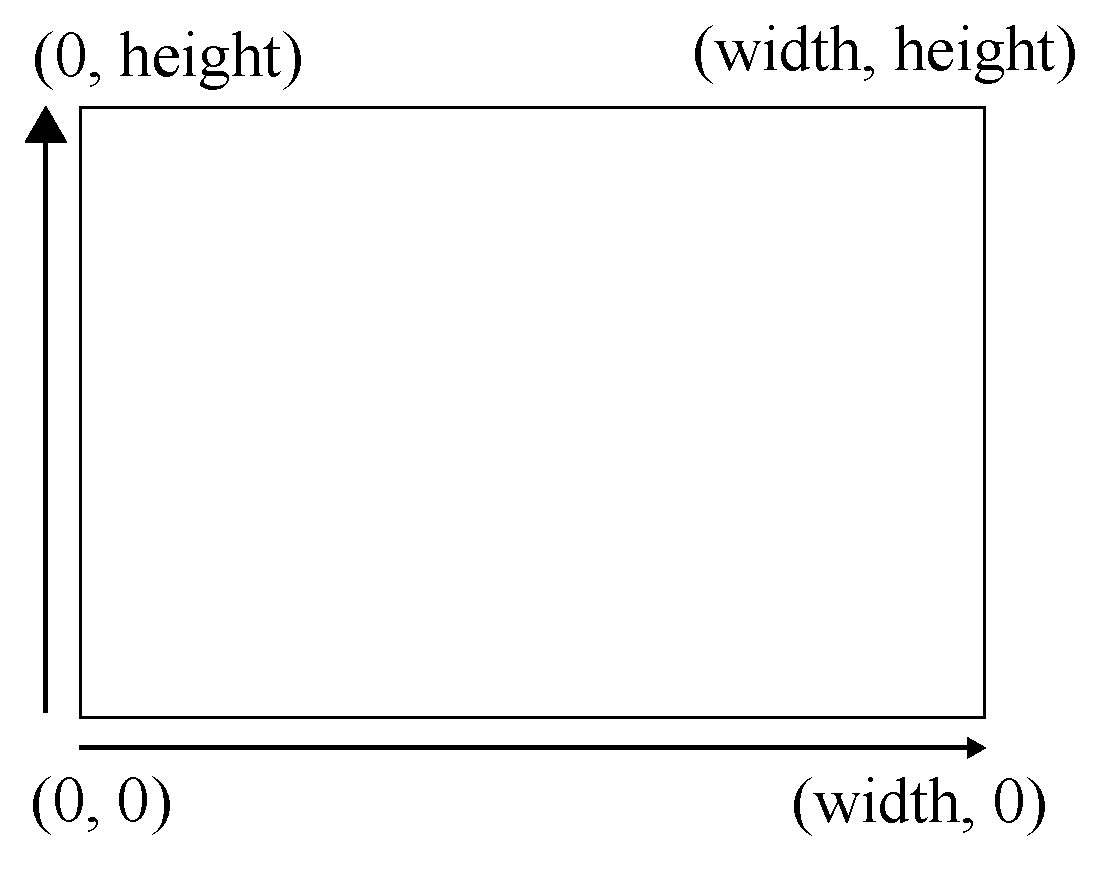
\includegraphics[width=\linewidth]{imgs/canvas.pdf}
        \caption{\label{fig:canvas}}
    \end{subfigure}
    \begin{subfigure}[t]{0.4\linewidth}
        \centering
        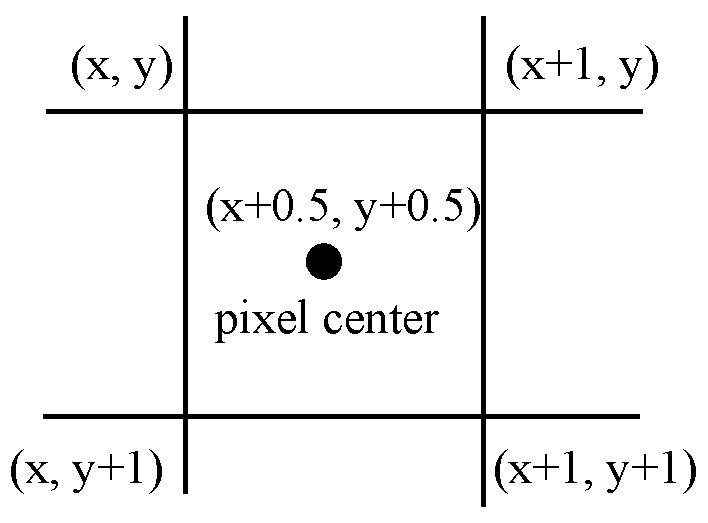
\includegraphics[width=\linewidth]{imgs/pixel.pdf}
        \caption{\label{fig:pixel}}
    \end{subfigure}
    \caption{(a) The coordinate system of the ``canvas'' we will draw our shapes on. (b) The pixel center of for pixel $(x, y)$ locates at $(x+0.5, y+0.5)$.}
\end{figure}

In the first part of this homework, we will render a single circle on our image. We are given a white ``canvas'' (\cref{fig:canvas}), where in this part we assume it to be of size $640 \times 480$. We need a \textbf{coordinate system} to talk about points on this canvas. The usualy convention for an image is that the top left is the origin, and the x-axis points towards right, and the y-axis points downwards. We are futher given the center, radius, and color of the circle. These are command line arguments that we will parse for you.

To render an image, we need to determine the color for each pixel. For this part, we focus on determining the color of the center of the pixel (\cref{fig:pixel}). To determine the pixel color, we decide whether the pixel center hits the circle or not. If it hits the circle, then we decide that the pixel's color is the circle's color. Otherwise, we decide that the pixel's color is the background color (by default, let's say it's $(1, 1, 1)$). How to decide whether the pixel center hits the circle? That's for you to figure out!

Balboa provides a few utitilies that will be useful for this homework: \lstinline{Vector2}, \lstinline{Vector3}, and \lstinline{Image3}. They are defined in \lstinline{vector.h} and \lstinline{image.h}. 

\paragraph{Vectors.} \lstinline{Vector2} and \lstinline{Vector3} are utilities for representing 2D and 3D vectors. You can access their members using \lstinline{.x}, \lstinline{.y}, and \lstinline{.z}. We overloaded a few common operators so that you can add and subtract vectors, and multiply them with scalars:
\begin{lstlisting}[language=C++]
Vector2 v0 = ..., v1 = ...;
v0 + v1; // vector addition
v0 - v1; // subtraction
v0 * Real(0.5) // multiply by a scalar
v0 / Real(0.5) // divide by a scalar
dot(v0, v1) // dot product between the two vectors
normalize(v0) // returns a vector with same direction as v0, but with magnitude of 1
\end{lstlisting}
In balboa, we represent floating point numbers using the type \lstinline{Real}. It is by default defined to be a \lstinline{double}. It is designed such that when you want to switch to single precision float (maybe for less memory cost), you can switch a single line in \lstinline{balboa.h}.
\begin{lstlisting}[language=C++]
using Real = double;
\end{lstlisting}

\begin{figure}[h]
    \centering
    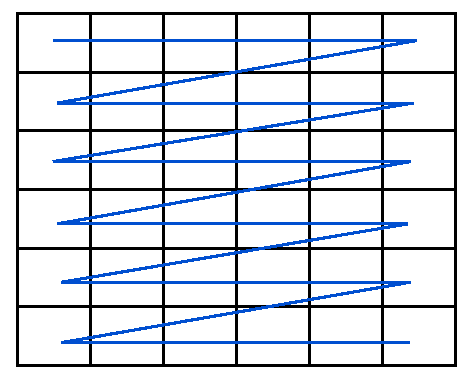
\includegraphics[width=0.4\linewidth]{imgs/scanline.pdf}
    \caption{Storing a 2D image in an 1D array by scanning the image.}
    \label{fig:scanline}
\end{figure}

\paragraph{Images.} \lstinline{Image3} represents a 3-channel raster image (usually storing red, green, blue value at each channel respectively). We store the 2D image in a 1D array using a scanline (\cref{fig:scanline}). You can access the 2D image using the \lstinline{()} operator:
\begin{lstlisting}[language=C++]
Image3 img(640 /* width */, 480 /* height */);
Vector3 val = img(50, 20); // reading values from location (50, 20)
img(30, 60) = Vector3{0.5, 0.6, 0.7}; // writing values to location (30, 60)
img.width; // 640
img.height; // 480
imwrite("image.png", img); // write the image to the disk
Image3 img2 = imread3("image2.png"); // read an image from the disk
\end{lstlisting}
The pixel values are stored as \lstinline{Real} in the memory. When we write the image into a file, the file format can often only supports 8-bit integers. The conversion is made in the \lstinline{imwrite} function, where we apply a \href{https://en.wikipedia.org/wiki/Gamma_correction}{gamma correction} to encode the image (with $\gamma=\frac{1}{2.2}$). We will likely talk about gamma correction in the class.

You should be ready to implement the circle rendering code in \lstinline{hw_1_1} in \lstinline{hw1.cpp} at this point. 
To see your results, in terminal, type:
\begin{lstlisting}[language=bash]
  ./balboa -hw 1_1 -center 200 300 -radius 100 -color 0.3 0.7 0.5
  ./balboa -hw 1_1 -center -50 250 -radius 100 -color 0.7 0.3 0.3
  ./balboa -hw 1_1 -center 600 250 -radius 150 -color 0.3 0.5 0.7
  ./balboa -hw 1_1 -center 250 470 -radius 50 -color 0.7 0.5 0.7
\end{lstlisting}
or just any parameter you like! \cref{fig:hw1_1} shows our rendering for the first command.

\begin{figure}[ht]
    \centering
    
\includegraphics[width=0.5\linewidth]{imgs/hw_1_1.png}
    \caption{References for Homework 1.1.}
    \label{fig:hw1_1}
\end{figure}

If you see your circles, congratulations! If you have not done graphics-related stuff before, this is likely the first time you have use code to generate an image from scratch. This is what makes computer graphics fun at least for me: you paint on a canvas using code (and sometimes math) instead of a brush. This makes people who are not that good in traditional art capable of generating beautiful pictures (yes, the images you generate will become prettier from now on). Furthermore, unlike things like Stable Diffusion, you maintain full control of the process: at this point, you know exactly how each pixel is generated, and if you don't like it, it's very easy to fix if you know how computer graphics works.

\section{Rendering multiple circles (10 pts)}

In this part, we will extend our previous code to handle multiple circles. This mostly boils down to adding a for loop to check over all of the circles for all of the pixels. However, things become more interesting here: it turns out there are two ways to structure the loops:
\begin{lstlisting}[language=Python]
# For each pixel, check all circles
for each pixel:
    for each circle:
        # check if the pixel center hits the circle
        # overwrite color if the circle is closer

# For each circle, check all pixels
for each circle:
    for each pixel:
        # check if the pixel center hits the circle
        # overwrite color if the circle is closer
\end{lstlisting}
Think for a bit: do these two produce the same results? The first loop structure finds the closest hitting circle for each pixel, and the second loop structure \emph{paints} each circle on the canvas in order. It will be clearer in the future lectures that in 3D graphics, the first loop structure is usually called \emph{ray tracing} (or ray casting) and the second loop structure is called \emph{rasterization}.

Another small complication we need to resolve is to decide which circle is the closest when there are multiple ones overlapping with a pixel. We simply assume the circles are ordered from the farthest to the closest. 

For this part, you can choose to implement either style above that suits you better. The scene is given in the array \lstinline{hw1_2_scenes} in \lstinline{hw1_scenes.h}. Note that the scene also specifies the background color and the canvas resolution. We will select the scenes using command line arguments. Implement your rendering code in the function \lstinline{hw_1_2} and see the result using the following commands:
\begin{lstlisting}[language=bash]
  ./balboa -hw 1_2 [scene_id]
\end{lstlisting}
where \lstinline{[scene_id]} is the scene you want to render (0-4).

We show our rendering for scene 0 in \cref{fig:hw1_2}. We will grade your results using the other scenes.

\begin{figure}[ht]
    \begin{minipage}{0.67\linewidth}
    \centering
    
\includegraphics[width=\linewidth]{imgs/hw_1_2.png}
    \caption{References for Homework 1.2.}
    \label{fig:hw1_2}
    \end{minipage}
    \begin{minipage}{0.32\linewidth}
    \centering
    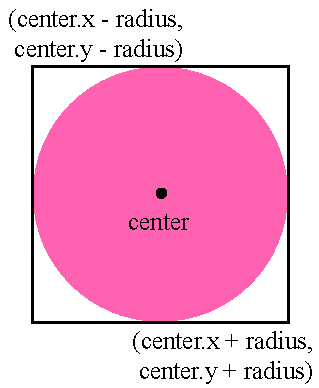
\includegraphics[width=\linewidth]{imgs/circle_box.pdf}
    \caption{The axis-aligned bounding box of a circle.}
    \label{fig:circle_box}
    \end{minipage}
\end{figure}

\paragraph{Bonus: accelerating rasterization using bounding boxes.} In practice, we may have a lot of circles and a lot of pixels. So we want to pick a way to render that is the fastest. Both loop structures can be sped up significantly. The observation is that most of the time, each pixel would only hits a small amount of circles. Or equivalently, each circle only will overlap with a small amount of pixels. It turns out that the acceleration for the first loop structure (ray tracing) is a bit more involved (we will discuss them in \href{https://cseweb.ucsd.edu/~tzli/cse168}{CSE 168}), so we will only talk about the acceleration for the rasterization part.

Notice that each circle usually only intersect with a small set of pixels. Therefore, we can modify the rasterization loop into the following:
\begin{lstlisting}[language=Python]
# For each circle, check all pixels
for each circle:
    bounding_box = \
        BBox(circle.center - radius,
             circle.center + radius)
    for each pixel in bounding_box:
        # check if the pixel center hits the circle
        # overwrite color if the circle is closer
\end{lstlisting}
Here, for each circle, we can compute an \emph{axis-aligned bounding box} that contains the circle (\cref{fig:circle_box}), and only loop over the pixels that overlaps with the bounding box. An axis-aligned bounding box is defined by two points: the point on the top left, and the point at the bottom right. 

For the bonus, implement the rasterization loop above, and report the speedup you obtain before and after the optimization.

\section{Rendering more shapes (10 pts)}

Next, we will add more types of shapes into our renderer. In particular, we will support rendering an (axis-aligned) rectangle and a triangle. Before that, let's introduce our scene file format, so that we don't have to hardcode our scenes in a C++ header. There is no a single standard way to represent a scene in computer graphics.\footnote{Though in 2D, \href{https://en.wikipedia.org/wiki/SVG}{Scalable Vector Graphics (SVG)} is the most popular, and in 3D, studios are converging towards the \href{https://en.wikipedia.org/wiki/Universal_Scene_Description}{Universal Scene Description}.} Thus, we will use an easily readable and parsible \href{https://en.wikipedia.org/wiki/JSON}{JSON} format to describe our scene. It's easiest to explain by showing scene 0 from the previous part in our scene format:
\begin{lstlisting}[language=json]
{
    "resolution": [640, 360],
    "background": [
        0.5, 0.5, 0.5
    ],
    "objects": [
        {
            "type": "circle",
            "center": [320, 180],
            "radius": 160,
            "color": [0.3, 0.5, 0.8]
        },
        {
            "type": "circle",
            "center": [150, 80],
            "radius": 80,
            "color": [0.8, 0.3, 0.5]
        },
        {
            "type": "circle",
            "center": [490, 80],
            "radius": 80,
            "color": [0.8, 0.3, 0.5]
        }
    ]
}
\end{lstlisting}

We will provide the scene parser for you. The scene is parsed into the following \lstinline{struct}:
\begin{lstlisting}[language=C++]
struct Scene {
    Vector2i resolution;
    Vector3 background;
    std::vector<Shape> shapes;
};
\end{lstlisting}
where \lstinline{Shape} is a \lstinline{std::variant}:
\begin{lstlisting}[language=C++]
struct Circle {
    Vector2 center;
    Real radius;
    Vector3 color;
};

struct Rectangle {
    Vector2 p_min, p_max;
    Vector3 color;
};

struct Triangle {
    Vector2 p0, p1, p2;
    Vector3 color;
};

using Shape = std::variant<Circle, Rectangle, Triangle>;
\end{lstlisting}

A \lstinline{std:variant} can be seen as a \emph{tagged union}:
\begin{lstlisting}[language=C++]
struct Foo {
  int type;
  union {
    Type0 t0;
    Type1 t1;
    // ...
  }
};
\end{lstlisting}
Read more about it \href{https://www.cppstories.com/2020/04/variant-virtual-polymorphism.html/}{here}. I used variant here so that I can store all shapes in a single linear array without separate heap memory allocation.

In your code, one way to deal with different types of \lstinline{Shape} could be the following:
\begin{lstlisting}[language=C++]
if (auto *circle = std::get_if<Circle>(&shape)) {
    // do something with circle
} else if (auto *rectangle = std::get_if<Rectangle>(&shape)) {
    // do something with rectangle
} else if (auto *triangle = std::get_if<Triangle>(&shape)) {
    // do something with triangle
}
\end{lstlisting}

A \lstinline{Rectangle} is axis-aligned and is defined by its top-left (\lstinline{p_min}) and bottom-right (\lstinline{p_max}) points. Testing whether a 2D point is inside an axis-aligned rectangle is easy and I'll leave it to you to figure it out.

\begin{figure}[t]
    \centering
    \begin{minipage}{0.5\linewidth}
    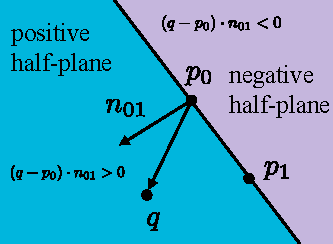
\includegraphics[width=\linewidth]{imgs/half_planes.pdf}
    \caption{Each edge of a triangle forms a line that splits the 2D space into two half planes. Here we show the edge from $p_0$ and $p_1$. The line has a ``normal'' direction $n_{01}$ that is perpendicular to the edge direction (i.e., $n_{01} \cdot \left(p_1 - p_0\right) = 0$). For a point $q$, we can determine which half-plane it is in by forming a vector with $p_0$ and taking dot product with $n_{01}$. If the dot product is positive, it is on the same side as where the normal is pointing at, and vice versa.}
    \label{fig:half_planes}
    \end{minipage}
    \hspace{20pt}
    \begin{minipage}{0.39\linewidth}
    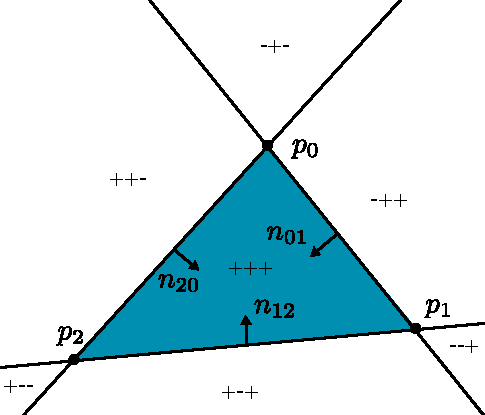
\includegraphics[width=\linewidth]{imgs/tri_half_planes.pdf}
    \caption{The 6 half-planes formed by the 3 edges split the 2D plane into 7 regions. If all normals are pointing inwards, then the interior of the triangle is the intersection of all three positive half-planes. Otherwise the interior is the intersection of all negative half-planes.}
    \label{fig:tri_half_planes}
    \end{minipage}
\end{figure}

A \lstinline{Triangle} is defined by three points (\lstinline{p0, p1} and \lstinline{p2}). Testing whether a point is inside a triangle is a bit more involved. There are more than one way to do it, but I like to do it by looking at the \emph{half-planes} formed by the three edges of a triangle. For each edge of the triangle, we can form a line that splits the whole 2D space into two parts, we call these parts half-planes (\cref{fig:half_planes}). We can determine whether a point $q$ is on the positive or negative half-planes by looking at the sign of the dot product between a vector formed by the point $q$ and the line, and a normal vector $n$ that is perpendicular to the direction of the line. 

The key observation for testing whether a point is inside a triangle or test, is to notice that if we follow the three edge directions: $p_1 - p_0$, $p_2 - p_1$, and $p_0 - p_2$, and rotate them by 90 degrees in clockwise direction to obtain the normals $n_{01}$, $n_{12}$, and $n_{20}$, then the interior of the triangle is the intersection of all the positive half-planes or all the negative half-planes. More precisely, if $p_0, p_1$ and $p_2$ follows the clockwise direction, then the interior would be the intersection of all the positive half-planes, otherwise if $p_0, p_1$ and $p_2$ follows the counterclockwise direction, then the interior would be the intersection of all the negative half-planes.

The remaining question is how do we rotate the edge directions to obtain the normals? Recall that the 2D counterclockwise rotation matrix is:
\begin{equation}
\begin{bmatrix}
\cos \theta & -\sin \theta \\
\sin \theta & \cos \theta
\end{bmatrix},
\end{equation}
where $\theta$ is the (counterclockwise) rotation angle -- plugging in $\theta = -90^{\circ}$ we obtain:
\begin{equation}
\begin{bmatrix}
0 & 1 \\
-1 & 0
\end{bmatrix}
\begin{bmatrix}
x \\ y
\end{bmatrix}
=
\begin{bmatrix}
y \\ -x
\end{bmatrix}.
\end{equation}

Thus, to obtain normal $n_{01}$, we can take the edge $e_{01} = p_1 - p_0$, and set $n_{01}.x = e_{01}.y$ and $n_{01}.y = -e_{01}.x$.

At this point, you should have enough knowledge to implement a renderer that can handle circles, rectangles, and triangles. Write your code in \lstinline{hw_1_3} and test it using the following commands:
\begin{lstlisting}[language=bash]
  ./balboa -hw 1_3 ../scenes/hw1/three_circles.json
  ./balboa -hw 1_3 ../scenes/hw1/three_shapes.json
\end{lstlisting}

We show our rendering of the \lstinline{three_shapes} scene in \cref{fig:hw1_3}. We will grade your results using other scenes.

\begin{figure}[ht]
    \centering
    
\includegraphics[width=0.5\linewidth]{imgs/hw_1_3.png}
    \caption{References for Homework 1.3.}
    \label{fig:hw1_3}
\end{figure}

\section{2D transformation (10 pts)}

\section{Alpha blending (10 pts)}


%\bibliographystyle{plain}
%\bibliography{refs}

\end{document}
